% =====================================================================
%  PeakCheck — User Manual (English)
%  Compile: pdflatex Manual_PeakCheck_EN.tex  (2x for references)
% =====================================================================
\documentclass[11pt,a4paper]{article}
\def\peakchecklang{english}
% =====================================================================
%  PeakCheck — shared LaTeX preamble
%  Used by:  Anleitung_PeakCheck.tex (DE), Manual_PeakCheck_EN.tex (EN),
%            Supplement_PeakCheck_EN.tex (EN)
%
%  Set the document language BEFORE % =====================================================================
%  PeakCheck — shared LaTeX preamble
%  Used by:  Anleitung_PeakCheck.tex (DE), Manual_PeakCheck_EN.tex (EN),
%            Supplement_PeakCheck_EN.tex (EN)
%
%  Set the document language BEFORE % =====================================================================
%  PeakCheck — shared LaTeX preamble
%  Used by:  Anleitung_PeakCheck.tex (DE), Manual_PeakCheck_EN.tex (EN),
%            Supplement_PeakCheck_EN.tex (EN)
%
%  Set the document language BEFORE \input{preamble.tex}, e.g.
%      \def\peakchecklang{english}   % or:  \def\peakchecklang{ngerman}
%  Engine: pdflatex.  Bibliography: bibtex + natbib (plainnat).
% =====================================================================

\usepackage[T1]{fontenc}
\usepackage[utf8]{inputenc}
\providecommand{\peakchecklang}{english}
% Graceful fallback: if the requested German babel files are absent (minimal
% TeX Live), fall back to english so the file still compiles. A full TeX Live /
% Overleaf has texlive-lang-german, so there the document stays German.
\def\pklangde{ngerman}
\ifx\peakchecklang\pklangde
  \IfFileExists{ngermanb.ldf}{}{\def\peakchecklang{english}}
\fi
\usepackage[\peakchecklang]{babel}
\IfFileExists{lmodern.sty}{\usepackage{lmodern}}{}

\usepackage[a4paper,margin=2.3cm]{geometry}
\usepackage{amsmath}
\usepackage{amssymb}
\usepackage{mathtools}
\usepackage{graphicx}
\usepackage{xcolor}
\usepackage{listings}
\usepackage{booktabs}
\usepackage{array}
\usepackage{tabularx}
\usepackage{ragged2e}
\usepackage{enumitem}
\usepackage{caption}
\usepackage[numbers,sort&compress]{natbib}
\IfFileExists{microtype.sty}{\usepackage[protrusion=true,expansion=false]{microtype}}{}

% hyperref last
\usepackage[colorlinks=true,linkcolor=pkblue,citecolor=pkblue,urlcolor=pkblue]{hyperref}

% --- colours ---------------------------------------------------------
\definecolor{pkblue}{HTML}{1F4E79}
\definecolor{pkaccent}{HTML}{C55A11}
\definecolor{codebg}{HTML}{F4F6F8}
\definecolor{codeframe}{HTML}{D6DEE6}
\definecolor{kw}{HTML}{0B5394}
\definecolor{str}{HTML}{7F6000}
\definecolor{cmt}{HTML}{6A737D}
\definecolor{hdrgray}{HTML}{555555}

% --- captions --------------------------------------------------------
\captionsetup{font=small,labelfont=bf,labelsep=period}

% --- listings: Python -----------------------------------------------
\lstdefinestyle{py}{%
  language=Python,
  basicstyle=\ttfamily\footnotesize,
  keywordstyle=\color{kw}\bfseries,
  stringstyle=\color{str},
  commentstyle=\color{cmt}\itshape,
  numberstyle=\tiny\color{cmt},
  backgroundcolor=\color{codebg},
  frame=single,
  framerule=0.4pt,
  rulecolor=\color{codeframe},
  showstringspaces=false,
  breaklines=true,
  breakatwhitespace=true,
  columns=fullflexible,
  keepspaces=true,
  tabsize=4,
  xleftmargin=10pt,
  xrightmargin=4pt,
  aboveskip=2pt,
  belowskip=10pt,
}

% --- listings: TOML / console (generic, '#' comments) ---------------
\lstdefinestyle{conf}{%
  basicstyle=\ttfamily\footnotesize,
  keywordstyle=\color{kw},
  commentstyle=\color{cmt}\itshape,
  morecomment=[l]{\#},
  morestring=[b]",
  stringstyle=\color{str},
  backgroundcolor=\color{codebg},
  frame=single,
  framerule=0.4pt,
  rulecolor=\color{codeframe},
  showstringspaces=false,
  breaklines=true,
  columns=fullflexible,
  keepspaces=true,
  xleftmargin=10pt,
  xrightmargin=4pt,
  aboveskip=2pt,
  belowskip=10pt,
}

% --- helper macros ---------------------------------------------------
% inline monospace (detokenize so _, #, & etc. need no escaping)
\newcommand{\code}[1]{\texttt{\detokenize{#1}}}
% header line shown above a code listing: module path + function
\newcommand{\codehdr}[1]{\par\smallskip\noindent
  {\small\ttfamily\color{hdrgray}#1}\par\nobreak\vspace{1pt}}
% a "source / code reference" margin-style note inline
\newcommand{\srcref}[1]{\textnormal{\small\color{hdrgray}(#1)}}

% nicer default spacing for itemize
\setlist[itemize]{leftmargin=1.4em,topsep=2pt,itemsep=1pt}
\setlist[enumerate]{leftmargin=1.6em,topsep=2pt,itemsep=2pt}

% table helpers
\newcolumntype{L}{>{\RaggedRight\arraybackslash}X}
\renewcommand{\arraystretch}{1.15}

% section formatting (lightweight; optional package)
\IfFileExists{sectsty.sty}{\usepackage{sectsty}\allsectionsfont{\color{pkblue}}}{}

\setlength{\parskip}{0.4em}
\setlength{\parindent}{0pt}
, e.g.
%      \def\peakchecklang{english}   % or:  \def\peakchecklang{ngerman}
%  Engine: pdflatex.  Bibliography: bibtex + natbib (plainnat).
% =====================================================================

\usepackage[T1]{fontenc}
\usepackage[utf8]{inputenc}
\providecommand{\peakchecklang}{english}
% Graceful fallback: if the requested German babel files are absent (minimal
% TeX Live), fall back to english so the file still compiles. A full TeX Live /
% Overleaf has texlive-lang-german, so there the document stays German.
\def\pklangde{ngerman}
\ifx\peakchecklang\pklangde
  \IfFileExists{ngermanb.ldf}{}{\def\peakchecklang{english}}
\fi
\usepackage[\peakchecklang]{babel}
\IfFileExists{lmodern.sty}{\usepackage{lmodern}}{}

\usepackage[a4paper,margin=2.3cm]{geometry}
\usepackage{amsmath}
\usepackage{amssymb}
\usepackage{mathtools}
\usepackage{graphicx}
\usepackage{xcolor}
\usepackage{listings}
\usepackage{booktabs}
\usepackage{array}
\usepackage{tabularx}
\usepackage{ragged2e}
\usepackage{enumitem}
\usepackage{caption}
\usepackage[numbers,sort&compress]{natbib}
\IfFileExists{microtype.sty}{\usepackage[protrusion=true,expansion=false]{microtype}}{}

% hyperref last
\usepackage[colorlinks=true,linkcolor=pkblue,citecolor=pkblue,urlcolor=pkblue]{hyperref}

% --- colours ---------------------------------------------------------
\definecolor{pkblue}{HTML}{1F4E79}
\definecolor{pkaccent}{HTML}{C55A11}
\definecolor{codebg}{HTML}{F4F6F8}
\definecolor{codeframe}{HTML}{D6DEE6}
\definecolor{kw}{HTML}{0B5394}
\definecolor{str}{HTML}{7F6000}
\definecolor{cmt}{HTML}{6A737D}
\definecolor{hdrgray}{HTML}{555555}

% --- captions --------------------------------------------------------
\captionsetup{font=small,labelfont=bf,labelsep=period}

% --- listings: Python -----------------------------------------------
\lstdefinestyle{py}{%
  language=Python,
  basicstyle=\ttfamily\footnotesize,
  keywordstyle=\color{kw}\bfseries,
  stringstyle=\color{str},
  commentstyle=\color{cmt}\itshape,
  numberstyle=\tiny\color{cmt},
  backgroundcolor=\color{codebg},
  frame=single,
  framerule=0.4pt,
  rulecolor=\color{codeframe},
  showstringspaces=false,
  breaklines=true,
  breakatwhitespace=true,
  columns=fullflexible,
  keepspaces=true,
  tabsize=4,
  xleftmargin=10pt,
  xrightmargin=4pt,
  aboveskip=2pt,
  belowskip=10pt,
}

% --- listings: TOML / console (generic, '#' comments) ---------------
\lstdefinestyle{conf}{%
  basicstyle=\ttfamily\footnotesize,
  keywordstyle=\color{kw},
  commentstyle=\color{cmt}\itshape,
  morecomment=[l]{\#},
  morestring=[b]",
  stringstyle=\color{str},
  backgroundcolor=\color{codebg},
  frame=single,
  framerule=0.4pt,
  rulecolor=\color{codeframe},
  showstringspaces=false,
  breaklines=true,
  columns=fullflexible,
  keepspaces=true,
  xleftmargin=10pt,
  xrightmargin=4pt,
  aboveskip=2pt,
  belowskip=10pt,
}

% --- helper macros ---------------------------------------------------
% inline monospace (detokenize so _, #, & etc. need no escaping)
\newcommand{\code}[1]{\texttt{\detokenize{#1}}}
% header line shown above a code listing: module path + function
\newcommand{\codehdr}[1]{\par\smallskip\noindent
  {\small\ttfamily\color{hdrgray}#1}\par\nobreak\vspace{1pt}}
% a "source / code reference" margin-style note inline
\newcommand{\srcref}[1]{\textnormal{\small\color{hdrgray}(#1)}}

% nicer default spacing for itemize
\setlist[itemize]{leftmargin=1.4em,topsep=2pt,itemsep=1pt}
\setlist[enumerate]{leftmargin=1.6em,topsep=2pt,itemsep=2pt}

% table helpers
\newcolumntype{L}{>{\RaggedRight\arraybackslash}X}
\renewcommand{\arraystretch}{1.15}

% section formatting (lightweight; optional package)
\IfFileExists{sectsty.sty}{\usepackage{sectsty}\allsectionsfont{\color{pkblue}}}{}

\setlength{\parskip}{0.4em}
\setlength{\parindent}{0pt}
, e.g.
%      \def\peakchecklang{english}   % or:  \def\peakchecklang{ngerman}
%  Engine: pdflatex.  Bibliography: bibtex + natbib (plainnat).
% =====================================================================

\usepackage[T1]{fontenc}
\usepackage[utf8]{inputenc}
\providecommand{\peakchecklang}{english}
% Graceful fallback: if the requested German babel files are absent (minimal
% TeX Live), fall back to english so the file still compiles. A full TeX Live /
% Overleaf has texlive-lang-german, so there the document stays German.
\def\pklangde{ngerman}
\ifx\peakchecklang\pklangde
  \IfFileExists{ngermanb.ldf}{}{\def\peakchecklang{english}}
\fi
\usepackage[\peakchecklang]{babel}
\IfFileExists{lmodern.sty}{\usepackage{lmodern}}{}

\usepackage[a4paper,margin=2.3cm]{geometry}
\usepackage{amsmath}
\usepackage{amssymb}
\usepackage{mathtools}
\usepackage{graphicx}
\usepackage{xcolor}
\usepackage{listings}
\usepackage{booktabs}
\usepackage{array}
\usepackage{tabularx}
\usepackage{ragged2e}
\usepackage{enumitem}
\usepackage{caption}
\usepackage[numbers,sort&compress]{natbib}
\IfFileExists{microtype.sty}{\usepackage[protrusion=true,expansion=false]{microtype}}{}

% hyperref last
\usepackage[colorlinks=true,linkcolor=pkblue,citecolor=pkblue,urlcolor=pkblue]{hyperref}

% --- colours ---------------------------------------------------------
\definecolor{pkblue}{HTML}{1F4E79}
\definecolor{pkaccent}{HTML}{C55A11}
\definecolor{codebg}{HTML}{F4F6F8}
\definecolor{codeframe}{HTML}{D6DEE6}
\definecolor{kw}{HTML}{0B5394}
\definecolor{str}{HTML}{7F6000}
\definecolor{cmt}{HTML}{6A737D}
\definecolor{hdrgray}{HTML}{555555}

% --- captions --------------------------------------------------------
\captionsetup{font=small,labelfont=bf,labelsep=period}

% --- listings: Python -----------------------------------------------
\lstdefinestyle{py}{%
  language=Python,
  basicstyle=\ttfamily\footnotesize,
  keywordstyle=\color{kw}\bfseries,
  stringstyle=\color{str},
  commentstyle=\color{cmt}\itshape,
  numberstyle=\tiny\color{cmt},
  backgroundcolor=\color{codebg},
  frame=single,
  framerule=0.4pt,
  rulecolor=\color{codeframe},
  showstringspaces=false,
  breaklines=true,
  breakatwhitespace=true,
  columns=fullflexible,
  keepspaces=true,
  tabsize=4,
  xleftmargin=10pt,
  xrightmargin=4pt,
  aboveskip=2pt,
  belowskip=10pt,
}

% --- listings: TOML / console (generic, '#' comments) ---------------
\lstdefinestyle{conf}{%
  basicstyle=\ttfamily\footnotesize,
  keywordstyle=\color{kw},
  commentstyle=\color{cmt}\itshape,
  morecomment=[l]{\#},
  morestring=[b]",
  stringstyle=\color{str},
  backgroundcolor=\color{codebg},
  frame=single,
  framerule=0.4pt,
  rulecolor=\color{codeframe},
  showstringspaces=false,
  breaklines=true,
  columns=fullflexible,
  keepspaces=true,
  xleftmargin=10pt,
  xrightmargin=4pt,
  aboveskip=2pt,
  belowskip=10pt,
}

% --- helper macros ---------------------------------------------------
% inline monospace (detokenize so _, #, & etc. need no escaping)
\newcommand{\code}[1]{\texttt{\detokenize{#1}}}
% header line shown above a code listing: module path + function
\newcommand{\codehdr}[1]{\par\smallskip\noindent
  {\small\ttfamily\color{hdrgray}#1}\par\nobreak\vspace{1pt}}
% a "source / code reference" margin-style note inline
\newcommand{\srcref}[1]{\textnormal{\small\color{hdrgray}(#1)}}

% nicer default spacing for itemize
\setlist[itemize]{leftmargin=1.4em,topsep=2pt,itemsep=1pt}
\setlist[enumerate]{leftmargin=1.6em,topsep=2pt,itemsep=2pt}

% table helpers
\newcolumntype{L}{>{\RaggedRight\arraybackslash}X}
\renewcommand{\arraystretch}{1.15}

% section formatting (lightweight; optional package)
\IfFileExists{sectsty.sty}{\usepackage{sectsty}\allsectionsfont{\color{pkblue}}}{}

\setlength{\parskip}{0.4em}
\setlength{\parindent}{0pt}


\title{\vspace{-1.5em}\color{pkblue}\bfseries PeakCheck --- User Manual\\[2pt]
\normalsize\mdseries\color{black}Interactive multi-peak fitting and
peak-presence checking for generic x/y data}
\author{Lukas Knauer\\[-2pt]
{\small RPTU Kaiserslautern-Landau \textperiodcentered\ AG Sch\"unemann}}
\date{\small Version 1.0.0 \textperiodcentered\ MIT license \textperiodcentered\ 2026}

\hypersetup{
  pdftitle={PeakCheck -- User Manual},
  pdfauthor={Lukas Knauer},
  pdfsubject={PeakCheck user manual: interactive multi-peak Voigt fitting and peak-presence checking},
  pdfkeywords={Voigt, peak fitting, spectroscopy, PeakCheck}
}

\begin{document}
\maketitle
\thispagestyle{empty}

\noindent\fcolorbox{codeframe}{codebg}{%
\parbox{\dimexpr\linewidth-2\fboxsep\relax}{\small
\textbf{What does PeakCheck do?} It determines peaks in a reference data set
(e.g.\ a summed spectrum) and then checks whether those same peaks are present in
one or more component data sets (e.g.\ sub-spectra). It works with any 2- or
3-column x/y data --- spectra, diffraction patterns, chromatograms, time series.}}

\begin{figure}[h]
\centering
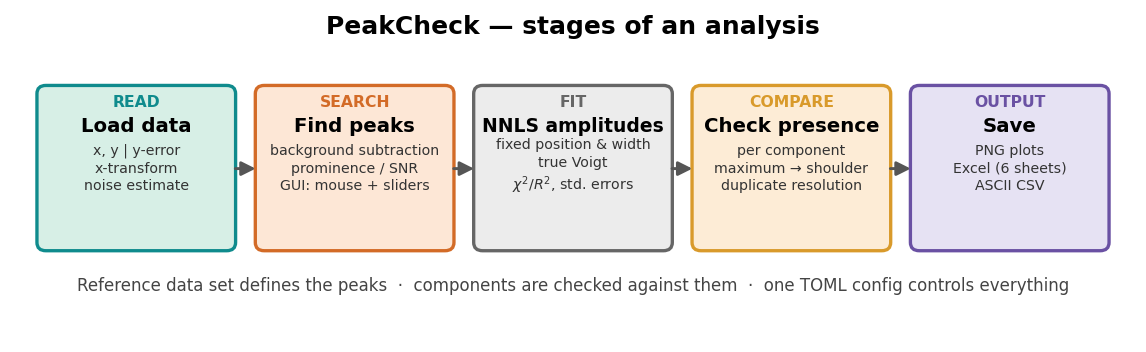
\includegraphics[width=0.88\linewidth]{figures/fig_pipeline.png}
\caption{The five stages of an analysis: read, search, fit, compare, output.}
\end{figure}

% =====================================================================
\section{Installation \& start}
PeakCheck is a small Python package with a backwards-compatible launcher
(\code{peakcheck.py}). It needs Python 3.10+ and the packages \code{numpy},
\code{scipy}, \code{matplotlib} and \code{openpyxl}, plus Tk for the graphical
interface.

\begin{lstlisting}[style=conf]
# Install the packages (once)
pip install numpy scipy matplotlib openpyxl
# Tk ships with the python.org installer on Windows/macOS; on Linux:
sudo apt install python3-tk
# For Python < 3.11 also the TOML reader:
pip install tomli
\end{lstlisting}

There are three equivalent ways to start it. Pick whichever fits your habits:

\begin{lstlisting}[style=conf]
# 1) Graphical (default): open a window, tune, click, fit & save
python -m peakcheck            # or simply: peakcheck   (after pip install)
python peakcheck.py            # still works as a backwards-compatible launcher

# 2) Headless, driven by a TOML file (batch / HPC)
python -m peakcheck --config job.toml --no-gui

# 3) Write a commented configuration template
python -m peakcheck --write-template job.toml
\end{lstlisting}

\noindent\textit{In Spyder, run it as a standalone program (not inside the
IPython console) so a real window opens; or set \code{\%matplotlib qt5} in the
console beforehand.}

% =====================================================================
\section{Input data}
PeakCheck reads plain-text column data regardless of the file extension:
\code{.dat}, \code{.txt}, \code{.csv}, \code{.xy}, \code{.asc}, \code{.tsv},
\code{.prn}, \code{.nis} and similar all work, as long as the file contains two
or three numeric columns. Values may be separated by whitespace, tabs, commas or
semicolons; header lines, comment characters (\code{# ! \%}) and a German-style
decimal comma (e.g.\ \code{10,5}) are detected and handled automatically. (The
one extension treated specially is \code{.fio}; see below.)

\begin{table}[h]\small\centering
\begin{tabularx}{\linewidth}{@{}l l L@{}}
\toprule
\textbf{Format} & \textbf{Meaning} & \textbf{Effect on the fit}\\
\midrule
\code{x  y} & two columns, no errors & unweighted fit; noise is estimated from the data\\
\code{x  y  y_error} & three columns with a measurement error & weighted fit; errors enter as $1/\sigma$\\
\bottomrule
\end{tabularx}
\end{table}

\noindent\textbf{FIO files (DESY/PETRA III).} Files ending in \code{.fio} are read
directly: PeakCheck parses the \code{\%d} data block with its \code{Col} column
declarations (the \code{\%c}/\code{\%p} comment and parameter blocks are ignored).
Because such files hold many columns, two settings choose which to use:
\code{fio_x_column} (default: the first column, typically the energy axis) and
\code{fio_y_column} (default \code{"nisp"}, the NIS signal). Either may be a column
\emph{name} (e.g.\ \code{"nfsp"}) or a 1-based index. FIO files carry no
per-point error column, so the noise is estimated unless you point
\code{error_column} at a specific column.
reference is \code{sample.txt}, then \code{sample_01.txt}, \code{sample_42.txt}
etc.\ are picked up as components. The pattern is configurable via
\code{component_glob}.

% =====================================================================
\section{The graphical interface}
\begin{figure}[h]
\centering
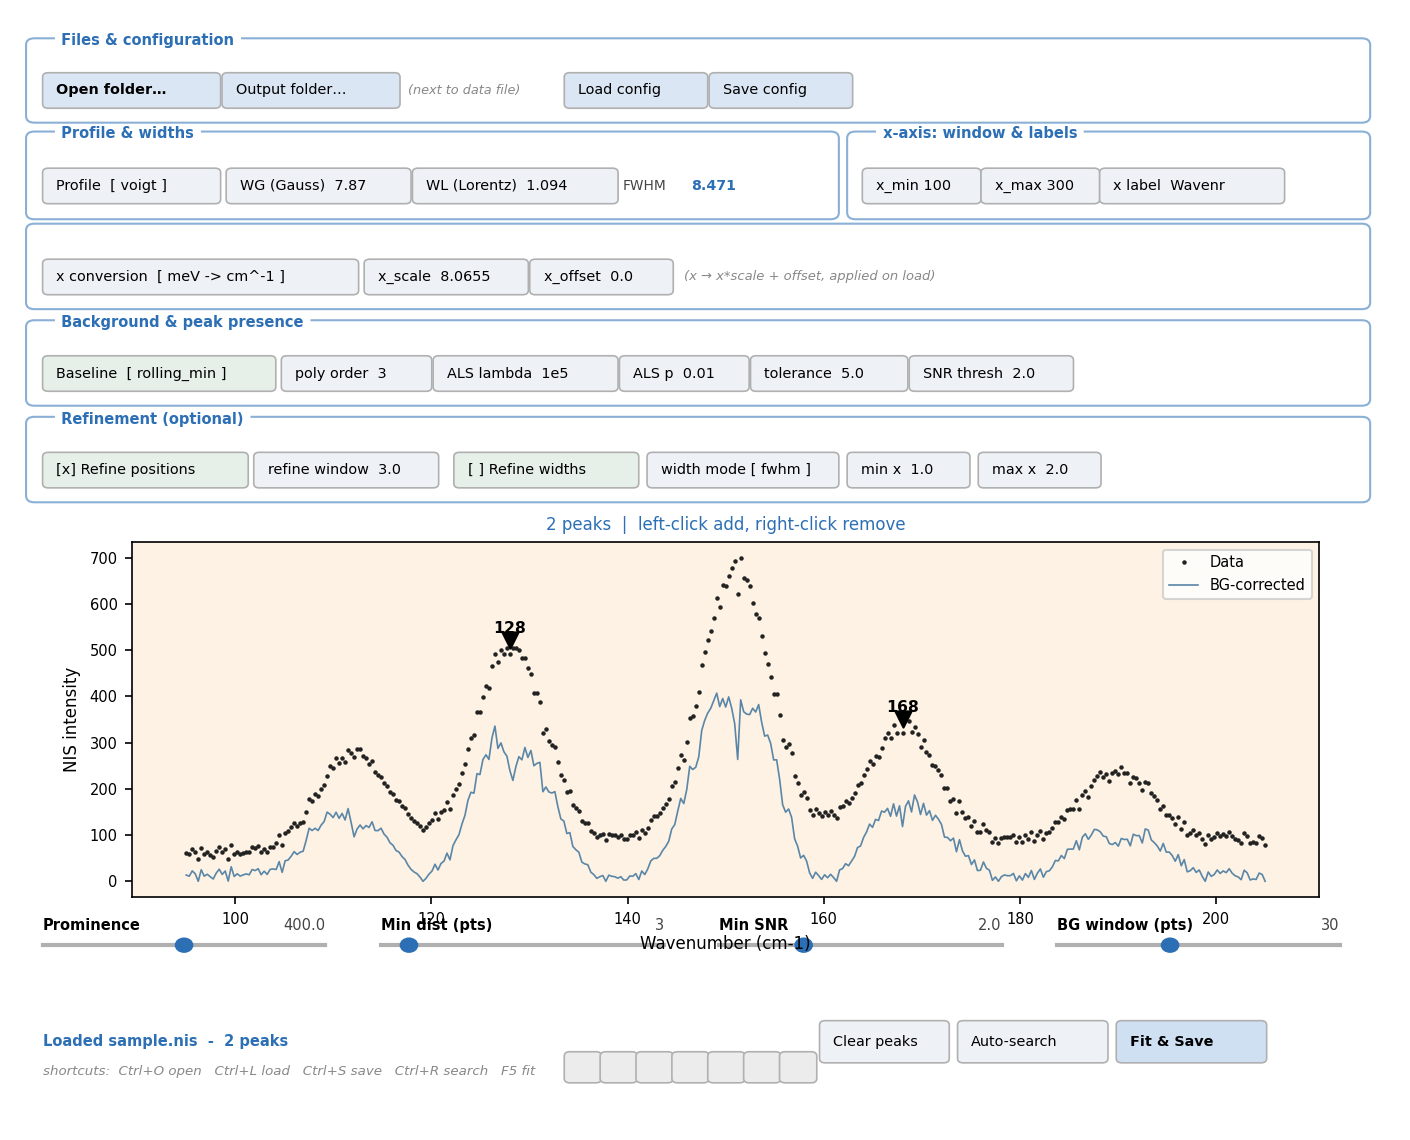
\includegraphics[width=0.92\linewidth]{figures/fig_gui.png}
\caption{The PeakCheck window: the controls are grouped into labelled frames
(Files \& configuration; Profile \& widths; x-axis window, labels \& conversion;
Background \& peak presence; Refinement), followed by the interactive plot with
peak markers, the search sliders, and the \emph{Fit \& Save} button. Keyboard
shortcuts are shown along the bottom. Fields that do not apply to the current
selection (e.g.\ the ALS parameters when the baseline is not ALS) are greyed out.}
\label{fig:gui}
\end{figure}

\noindent\textbf{Workflow}
\begin{enumerate}
\item \textbf{Open a folder} via \emph{Open folder\dots}. A dialog lists every
data file in the folder. Pick one as the reference (radio button in the ``Ref''
column) and any number as components (check boxes in the ``Cmp'' column). Confirm
with \emph{OK} --- the data appear at once together with the background-corrected
curve (blue).
\item \textbf{Restrict the search range} with \code{x_min}/\code{x_max} (confirm
with \emph{Enter}); the active range is shaded orange.
\item \textbf{Choose profile and widths}: \code{voigt}, \code{gauss} or
\code{lorentz}, plus the FWHMs \code{WG} (Gaussian) and \code{WL} (Lorentzian).
The resulting effective FWHM of the chosen profile is shown next to them as a
read-only value (it updates as you edit \code{WG}/\code{WL} or the profile).
\item \textbf{Find peaks} with the four sliders (prominence, minimum distance,
minimum SNR, background window) controlling the automatic search; what each one
does is explained under ``Choosing parameters'' below.
\item \textbf{Baseline and refinement} (fourth row, optional): choose the
\code{baseline_method} used by the fit (\code{rolling_min}, \code{polynomial} or
\code{als}, with the polynomial order and ALS $\lambda$/$p$ next to it), and tick
\emph{Refine positions} to refine the centres within \code{refine window} after
the fit. The defaults reproduce the previous behaviour.
\item \textbf{Refine by mouse} directly in the plot:
  \begin{itemize}
  \item \emph{Left click} --- add a peak at the nearest data point
  \item \emph{Right click} --- remove the nearest peak marker
  \end{itemize}
\item \textbf{Fit \& Save} runs the fit, the presence check across components, and
writes all outputs.
\end{enumerate}

\noindent\fcolorbox{codeframe}{codebg}{%
\parbox{\dimexpr\linewidth-2\fboxsep\relax}{\small
\textbf{Suggested order:} set the search range first, then adjust the background
window so the blue curve traces the peaks cleanly, then fine-tune minimum SNR
($\approx 2$) and prominence --- and finally add or remove individual peaks by
mouse.}}

\medskip
\noindent Via \emph{Save config} / \emph{Load config} all settings can be stored
to and reloaded from a TOML file, making every analysis reproducible.

\subsection{Converting the x-axis units}
The third control row converts the x-axis on load. The \emph{x conversion}
drop-down offers common conversions as presets; it sets \code{x_scale},
\code{x_offset} and the axis label/unit automatically. For NIS/NRVS pick
``meV $\to$ cm$^{-1}$'' --- the whole analysis then runs in cm$^{-1}$.

\begin{table}[h]\small\centering
\begin{tabularx}{\linewidth}{@{}l l L@{}}
\toprule
\textbf{Preset} & \textbf{factor (\code{x_scale})} & \textbf{typical use}\\
\midrule
meV $\to$ cm$^{-1}$ & 8.065544    & NIS/NRVS, pDOS\\
cm$^{-1}$ $\to$ meV & 0.12398419  & reverse\\
meV $\to$ THz       & 0.24179893  & THz / inelastic spectroscopy\\
cm$^{-1}$ $\to$ THz & 0.029979246 & FIR, phonons\\
eV $\to$ cm$^{-1}$  & 8065.544    & general energy axes\\
meV $\to$ K ($k_B$) & 11.604518   & thermal scale\\
\bottomrule
\end{tabularx}
\end{table}

The GUI presets are the linear (affine) conversions
$x \to x\cdot\code{x_scale} + \code{x_offset}$; you can also enter a custom factor
in \code{x_scale}/\code{x_offset}. Reciprocal conversions (wavelength
$\leftrightarrow$ wavenumber/energy, e.g.\ cm$^{-1} = 10^{7}/\lambda\,[\mathrm{nm}]$)
are non-linear and are available through the TOML file only (see \S4).

\smallskip
\noindent\textit{Important:} the conversion is applied on load. All other values
given in x units --- \code{x_min}, \code{x_max}, \code{wg}, \code{wl},
\code{tolerance} --- therefore refer to the already converted values (e.g.\
cm$^{-1}$, not meV).

% =====================================================================
\section{Command line}
Besides the GUI, PeakCheck has a small command line (the \code{peakcheck} console
script, equivalently \code{python -m peakcheck}):

\begin{table}[h]\small\centering
\begin{tabularx}{\linewidth}{@{}l L@{}}
\toprule
\textbf{Command} & \textbf{Effect}\\
\midrule
\code{peakcheck} & launch the graphical interface\\
\code{peakcheck --write-template job.toml} & write a commented config template and exit\\
\code{peakcheck --config job.toml --no-gui} & headless (batch) run; needs a config\\
\code{peakcheck --config job.toml --validate} & check a config and exit (non-zero exit on error)\\
\code{peakcheck --list-conversions} & list the x-axis presets and exit\\
\code{peakcheck --reference data.dat} & override the reference file from the config\\
\code{peakcheck --output-dir DIR} & write all outputs to \code{DIR} (batch; overrides \code{output_dir})\\
\code{peakcheck --version} & print the version\\
\code{peakcheck --debug} & on error, show the full traceback instead of a short message\\
\bottomrule
\end{tabularx}
\end{table}

\noindent A headless run writes exactly the same plots, Excel workbook and CSV as
the GUI, so a config saved from the GUI reproduces its result in batch. Use
\code{--validate} in scripts to fail fast on a malformed config. On a bad config
or data file the command prints a short \code{PeakCheck: …} message and exits
non-zero; add \code{--debug} to see the full Python traceback.

% =====================================================================
\section{A first analysis}
The package ships a ready-to-run example in \code{example_data/}.

\noindent\textbf{Headless, in one line} (from \code{example_data/}):
\begin{lstlisting}[style=py]
python -m peakcheck --config nis_example.toml --no-gui
\end{lstlisting}
PeakCheck loads the reference \code{sample.nis}, fits five peaks, checks the two
component files \code{sample_A.nis} and \code{sample_B.nis}, and writes the plots,
the Excel workbook and the CSV next to the data.

\noindent\textbf{Interactive:} start \code{peakcheck}, click \emph{Open folder\dots}
(Ctrl+O) and pick \code{sample.nis} as the reference, \code{sample_A.nis} and
\code{sample_B.nis} as components. Choose the \emph{x conversion}
\code{meV -> cm^-1}, press \emph{Auto-search peaks} (Ctrl+R) or click the peaks by
hand, then \emph{Fit \& Save} (F5); see Figure~\ref{fig:gui}.

\noindent The fit reproduces the amplitudes, $\chi^2_\nu\approx5.5$ and
$R^2\approx0.945$ from the supplement and reports which of the five peaks each
component contains.

% =====================================================================
\section{Configuration via TOML}
For batch runs and reproducible pipelines a TOML file controls every parameter. A
commented template is produced by
\code{python -m peakcheck --write-template job.toml}. The reference below lists
all available keys grouped by TOML section, with their default value, meaning and
a hint when to change them.

\paragraph{\code{[input]}}
\begin{table}[h]\small\centering
\begin{tabularx}{\linewidth}{@{}l l L@{}}
\toprule
\textbf{Key} & \textbf{Default} & \textbf{Meaning}\\
\midrule
\code{reference_file} & \code{"data.txt"} & Path to the reference file whose peaks are determined first. A relative path is resolved against the config file's own directory, so a config and its data stay portable (batch-friendly); absolute paths are used as given. A command-line \code{--reference} overrides this and keeps the usual shell (working-directory) semantics.\\
\code{component_glob} & \code{""} (empty) & Glob pattern for component files. Empty $=$ automatic \code{<stem>_*.<ext>} (e.g.\ \code{sample.nis} $\to$ \code{sample_A.nis}). Override with an explicit pattern (e.g.\ \code{"sub_*.dat"}); from the GUI the selection is passed in directly via the folder dialog.\\
\code{error_column} & \code{"auto"} & \code{"auto"} $=$ use the third column as the error if present, else estimate from data. \code{"none"} $=$ always estimate. Integer $=$ explicit 0-based column index.\\
\code{fio_x_column} & \code{""} & FIO files only: x column by name or 1-based index; empty $=$ first column.\\
\code{fio_y_column} & \code{"nisp"} & FIO files only: y column by name (e.g.\ \code{"nfsp"}) or 1-based index.\\
\bottomrule
\end{tabularx}
\end{table}

\paragraph{\code{[xaxis]}}
\begin{table}[h]\small\centering
\begin{tabularx}{\linewidth}{@{}l l L@{}}
\toprule
\textbf{Key} & \textbf{Default} & \textbf{Meaning}\\
\midrule
\code{x_conversion} & \code{""} (empty) & Named preset such as \code{"meV -> cm^-1"}, \code{"cm^-1 -> THz"} or \code{"nm -> eV (reciprocal)"}. Sets scale, offset, label and unit automatically. The TOML template lists all presets.\\
\code{x_transform} & \code{"affine"} & \code{"affine"}: $x' = x\cdot s + o$ (most energy units). \code{"reciprocal"}: $x' = s/x + o$ (e.g.\ wavelength $\to$ wavenumber).\\
\code{x_scale}, \code{x_offset} & 1.0, 0.0 & Manual scale factor and offset. Ignored when \code{x_conversion} is set.\\
\code{x_label}, \code{y_label} & \code{"x"}, \code{"y"} & Axis labels used in plots and result files.\\
\code{x_unit} & \code{""} (empty) & x-axis unit; shown in parentheses behind the label and in the Excel unit header row (Origin style).\\
\bottomrule
\end{tabularx}
\end{table}

\paragraph{\code{[profile]} --- line shape and widths}
\begin{table}[h]\small\centering
\begin{tabularx}{\linewidth}{@{}l l L@{}}
\toprule
\textbf{Key} & \textbf{Default} & \textbf{Meaning}\\
\midrule
\code{profile} & \code{"voigt"} & \code{"voigt"} (exact Gaussian$\otimes$Lorentzian convolution), \code{"gauss"}, \code{"lorentz"}. Voigt is the physically correct default for most spectroscopies.\\
\code{wg} & 7.8701 & Gaussian FWHM in x-units --- the instrumental resolution. For NIS at BL09XU (SPring-8): ${\sim}0.8$~meV $\approx 6.4$~cm$^{-1}$; at P01 (PETRA~III): see beamline spec.\\
\code{wl} & 1.094 & Lorentzian FWHM in x-units --- natural linewidth plus thermal contributions. For non-decaying phonons usually small compared to \code{wg}.\\
\bottomrule
\end{tabularx}
\end{table}

\paragraph{\code{[window]} --- search and fit window}
\begin{table}[h]\small\centering
\begin{tabularx}{\linewidth}{@{}l l L@{}}
\toprule
\textbf{Key} & \textbf{Default} & \textbf{Meaning}\\
\midrule
\code{x_min}, \code{x_max} & \code{""}, \code{""} & Lower and upper bound of the analysis window in x-units. Empty $=$ open (full file). Influences peak search and fit; appears in the output filename for traceability (e.g.\ \code{_100_200}).\\
\code{bg_window} & 30 & Window size for background subtraction (rolling minimum, in points). Rule of thumb: somewhat wider than a peak, much narrower than the baseline curvature. 0 disables it.\\
\code{baseline_method} & \code{rolling_min} & Baseline estimator used by the fit, statistics and presence check: \code{rolling_min} (default), \code{polynomial} or \code{als} (asymmetric least squares). The smooth alternatives suit curved baselines; \code{baseline_poly_order} (3), \code{baseline_als_lambda} ($10^5$) and \code{baseline_als_p} (0.01) tune them.\\
\bottomrule
\end{tabularx}
\end{table}

\paragraph{\code{[search]} --- automatic peak search}
\begin{table}[h]\small\centering
\begin{tabularx}{\linewidth}{@{}l l L@{}}
\toprule
\textbf{Key} & \textbf{Default} & \textbf{Meaning}\\
\midrule
\code{prominence_init} & 200.0 & Minimum prominence in y-units (\code{scipy.signal.find_peaks}). Higher values reject noise but miss weak peaks. Live-adjustable via slider in the GUI.\\
\code{distance_init} & 3 & Minimum distance between peaks in points. Prevents adjacent noise spikes from being counted as two peaks.\\
\code{min_snr_init} & 2.0 & SNR threshold for the auto-search (background-corrected signal). Accepts a peak only if its height $\ge \code{min_snr_init}\cdot$error.\\
\bottomrule
\end{tabularx}
\end{table}

\paragraph{\code{[refine]} --- optional position and width refinement}
Set \code{refine = true} to refine the peak positions after the fit by a bounded
nonlinear step (the amplitudes stay non-negative); \code{refine_window} (default
3.0, in x-units) limits how far each position may move. Set
\code{refine_widths = true} to additionally refine one width per peak:
\code{width_mode} chooses what broadens (\code{"fwhm"}, the default, scales the
whole Voigt; \code{"sigma"} scales only the Gaussian part), and the width is kept
within \code{width_min_factor}\,..\,\code{width_max_factor} times the instrumental
width (defaults 1.0\,..\,2.0, i.e.\ never narrower than the instrument and at most
twice as wide). Both are off by default, so the result is unchanged unless you
enable them.

\paragraph{\code{[presence]} --- presence check in components}
\begin{table}[h]\small\centering
\begin{tabularx}{\linewidth}{@{}l l L@{}}
\toprule
\textbf{Key} & \textbf{Default} & \textbf{Meaning}\\
\midrule
\code{tolerance} & 5.0 & $\pm$ position window in x-units within which a component peak counts as ``the same'' as a reference peak. Should be larger than the typical centroid shift between spectra, smaller than the peak spacing.\\
\code{snr_thresh} & 2.0 & SNR threshold above which a peak in the component counts as ``present''. Raise (4--6) for noisy spectra, lower (2--3) for clean spectra.\\
\code{presence_baseline_corrected} & \code{true} & \code{true} $=$ SNR measured on the background-corrected signal (height above baseline --- the physically meaningful value). \code{false} $=$ SNR on the raw data (includes background); rarely wanted.\\
\bottomrule
\end{tabularx}
\end{table}

\paragraph{\code{[errors]} --- error reporting}
\begin{table}[h]\small\centering
\begin{tabularx}{\linewidth}{@{}l l L@{}}
\toprule
\textbf{Key} & \textbf{Default} & \textbf{Meaning}\\
\midrule
\code{error_mode} & \code{"statistical"} & \code{"statistical"} $=$ true $1\sigma$ from $(B^{\top}W^2B)^{-1}$, unscaled (matches \code{absolute_sigma=True} in \code{scipy.curve_fit}). \code{"scaled"} $=$ multiplied by $\sqrt{\chi^2_\mathrm{red}}$ --- appropriate when only relative error weights are known.\\
\bottomrule
\end{tabularx}
\end{table}

\paragraph{\code{[output]}}
\begin{table}[h]\small\centering
\begin{tabularx}{\linewidth}{@{}l l L@{}}
\toprule
\textbf{Key} & \textbf{Default} & \textbf{Meaning}\\
\midrule
\code{output_dir} & \code{""} (empty) & Target folder for all outputs (plots, Excel, CSV). Empty $=$ next to the reference file. In the GUI also selectable via the ``Output folder\dots'' button.\\
\code{write_csv} & \code{true} & Write the ASCII CSV with all result sections. Setting to \code{false} keeps only the Excel file.\\
\code{write_excel} & \code{true} & Write the Excel workbook.\\
\code{plot_dpi} & 150 & Resolution of the saved PNG plots. 150 is fine for manuscript previews; raise to 300+ for print.\\
\bottomrule
\end{tabularx}
\end{table}

In addition the peak positions can be fixed directly instead of picking them
interactively or trusting the auto-search:
\begin{lstlisting}[style=conf]
peaks = [112.0, 128.0, 151.0, 168.0, 190.0]
\end{lstlisting}
The list is taken as the final set of peaks --- the auto-search is skipped
entirely. This is the most reproducible mode for manuscript pipelines.

% =====================================================================
\section{Choosing parameters \& good practice}
A short, practical guide; the supplement derives the reasoning.

\paragraph{Widths (\code{wg}, \code{wl}).} These are the \emph{instrumental}
resolution and are held fixed. Set them from the instrument/beamline, not from the
data. A reduced $\chi^2_\nu\gg1$ usually means the widths do not match the data (or
a peak is missing), not that the amplitudes are wrong.

\paragraph{Background (\code{baseline_method}).} The default rolling minimum is
robust for narrow peaks on a broad pedestal. For a smoothly curved background the
\code{polynomial} or \code{als} methods follow the curve more faithfully; ALS is
usually the best general choice (Figure~\ref{fig:baselines}). The same baseline is
used by the fit, the statistics and the presence check.

\begin{figure}[h]\centering
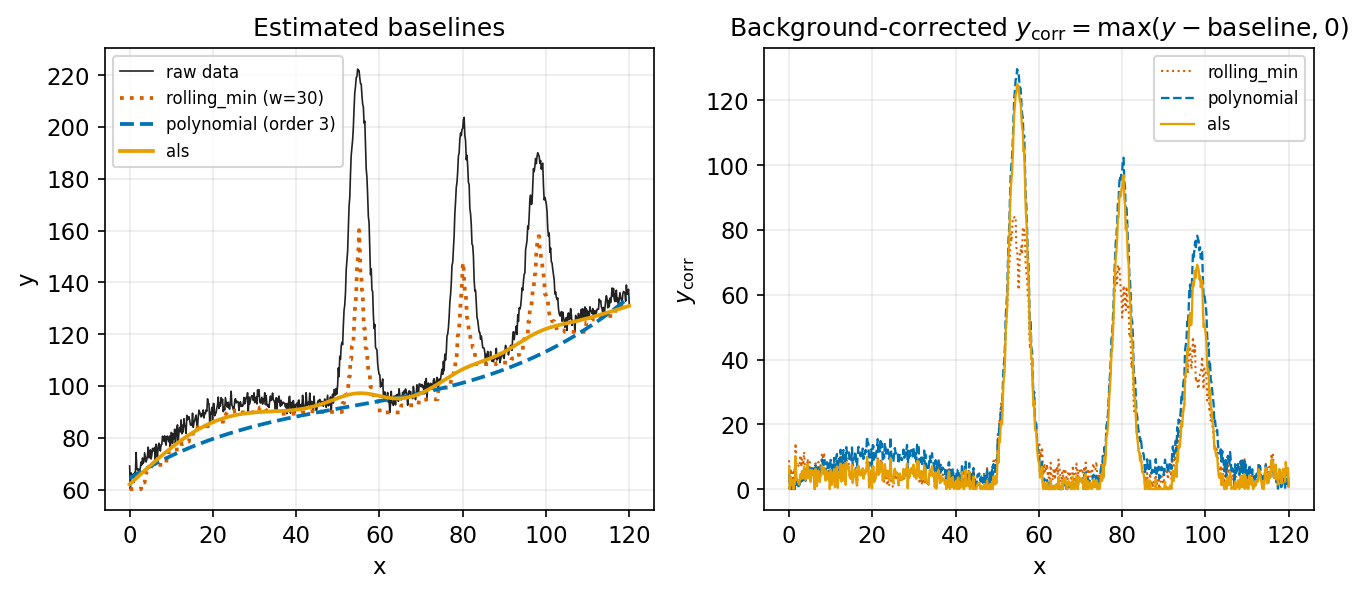
\includegraphics[width=\linewidth]{figures/fig_baselines.png}
\caption{The three baseline methods on one curved, noisy background. Left: the
estimated baselines --- the rolling minimum tracks the lower envelope in steps,
while the polynomial and ALS curves are smooth. Right: the corrected signal; ALS
and the polynomial flatten the background between the peaks more cleanly.}
\label{fig:baselines}
\end{figure}

\paragraph{The four search sliders.} The automatic search
(\code{scipy.signal.find_peaks} on the background-corrected signal) is driven by
four controls, all live in the GUI:
\begin{itemize}
\item \textbf{Prominence} (\code{prominence_init}, y-units): how far a peak must
  stand out from its local surroundings --- the height of the summit above the
  higher of its two neighbouring valleys, not the absolute y-value. This is the
  main control against noise: raise it to reject noise spikes, lower it to catch
  weak bands.
\item \textbf{Minimum distance} (\code{distance_init}, in data points): the
  smallest allowed separation between two detected peaks. It stops a noisy
  flank from being counted as several closely spaced peaks; when two candidates
  are closer than this, the more prominent one wins.
\item \textbf{Minimum SNR} (\code{min_snr_init}): a candidate is accepted only
  if its height is at least \code{min_snr_init} times the estimated noise. This
  complements prominence with a noise-relative criterion.
\item \textbf{Background window} (\code{bg_window}, in points): the window width
  of the background estimate (rolling minimum, or the chosen
  \code{baseline_method}) that is subtracted \emph{before} the search. Too small
  eats into real peaks; too large leaves a curved baseline standing; $0$ turns
  subtraction off. The same background feeds the fit and the presence check.
\end{itemize}
In the GUI you can also just click the peaks (left-click to add, right-click to
remove), which is often faster than fine-tuning the sliders.

\paragraph{Tolerance (\code{tolerance}).} The $\pm$ window in which a component peak
counts as ``the same'' as a reference peak. Make it larger than the typical
centroid shift between spectra but smaller than the peak spacing.

\paragraph{Position refinement (\code{refine}).} Off by default. Enable it when the
positions are slightly off (e.g.\ a small calibration shift): the centres are then
refined within \code{refine_window} while the amplitudes stay non-negative
(Figure~\ref{fig:refine}). Leave it off when the positions are known and trusted.

\begin{figure}[h]\centering
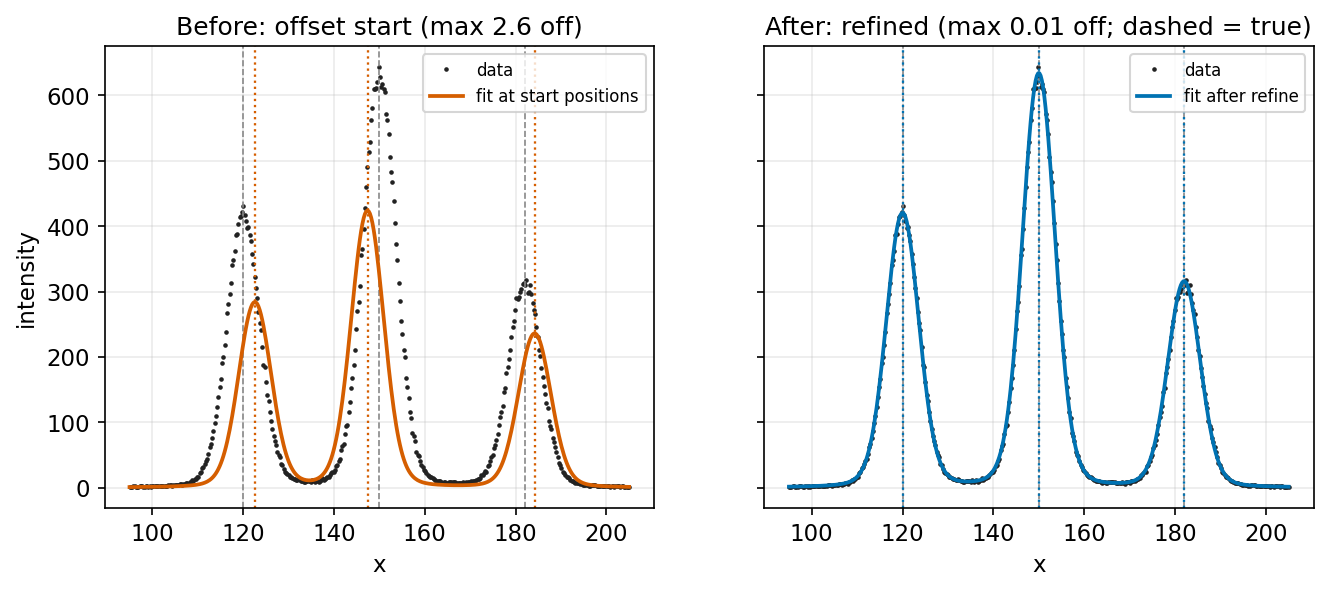
\includegraphics[width=\linewidth]{figures/fig_refine.png}
\caption{Optional position refinement. Left: a fit with deliberately offset start
positions (dotted) misses the true centres (dashed grey). Right: with
\code{refine = true} the centres are recovered to a small fraction of a point.}
\label{fig:refine}
\end{figure}

\paragraph{Width refinement (\code{refine_widths}).} Off by default; the widths
are otherwise held at the instrumental resolution for all peaks. Enable it when a
band is genuinely broader than the instrument (e.g.\ unresolved splitting or
inhomogeneous broadening). One width per peak is then refined, bounded between
\code{width_min_factor} and \code{width_max_factor} times the instrumental width;
\code{width_mode} selects whether the whole Voigt (\code{"fwhm"}) or only the
Gaussian part (\code{"sigma"}) broadens (Figure~\ref{fig:widths}). Keep the upper
bound tight: extra free widths always lower the reduced $\chi^2_\nu$ and, for
overlapping or weak peaks, width and amplitude trade off, so a smaller $\chi^2_\nu$
is not by itself evidence of a better model.

\begin{figure}[h]\centering
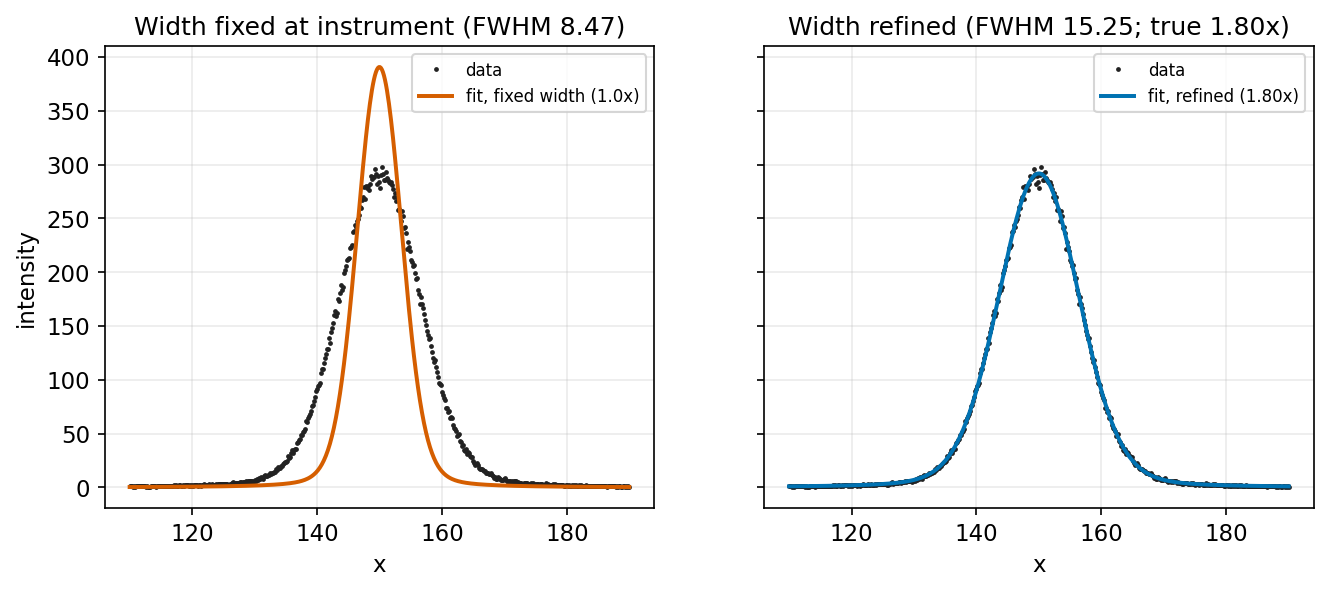
\includegraphics[width=\linewidth]{figures/fig_widths.png}
\caption{Optional per-peak width refinement on a peak that is genuinely broader
than the instrument. Left: with the width fixed at the instrumental resolution the
fit cannot reach the data. Right: with \code{refine_widths = true} the single
per-peak width is recovered (here a factor close to the true broadening), bounded
by \code{width_min_factor}\,..\,\code{width_max_factor}.}
\label{fig:widths}
\end{figure}

% =====================================================================
\section{Output files}
All results are written next to the reference file; an active search range appears
in the file name (e.g.\ \code{_90_200}).

\begin{table}[h]\small\centering
\begin{tabularx}{\linewidth}{@{}l L@{}}
\toprule
\textbf{File} & \textbf{Content}\\
\midrule
\code{*_fit.png} & fit with individual components and a residual panel\\
\code{*_peaks.png} & one marked plot per component (green $=$ present, red $=$ absent)\\
\code{*_results.xlsx} & Excel with six sheets: Intensities, Positions, Presence, Fit\_Data, Components\_Raw, Parameters (Components\_Raw only when components are analysed)\\
\code{*_results.csv} & a single plain 7-bit ASCII CSV with five labelled sections (Intensities, Positions, Presence, Fit\_Data, Components\_Raw) and the full parameter block as a header\\
\bottomrule
\end{tabularx}
\end{table}

The \code{Presence} sheet is the key result: a binary matrix showing $1$ (green,
present) or $0$ (red, absent) for each peak and component. The \code{Parameters}
sheet documents every run in full, keeping it reproducible.

\paragraph{Reading the plots.} Figures~\ref{fig:fit_annot} and
\ref{fig:presence_annot} label the two plot types. In the fit plot the black curve
is the sum, the coloured curves are the individual peaks (each area is the fitted
amplitude), and the lower panel shows the residuals --- a good fit leaves them
scattered around zero with no structure, and the title reports
$\chi^2_\nu$, $R^2$ and how many peaks ended up active. In a component plot a green
dashed line with a marker means the peak is present ($1$); a red dashed line means
it is absent ($0$). The decision is taken within the $\pm$\code{tolerance} window
(shaded) using the SNR threshold.

\begin{figure}[h]\centering
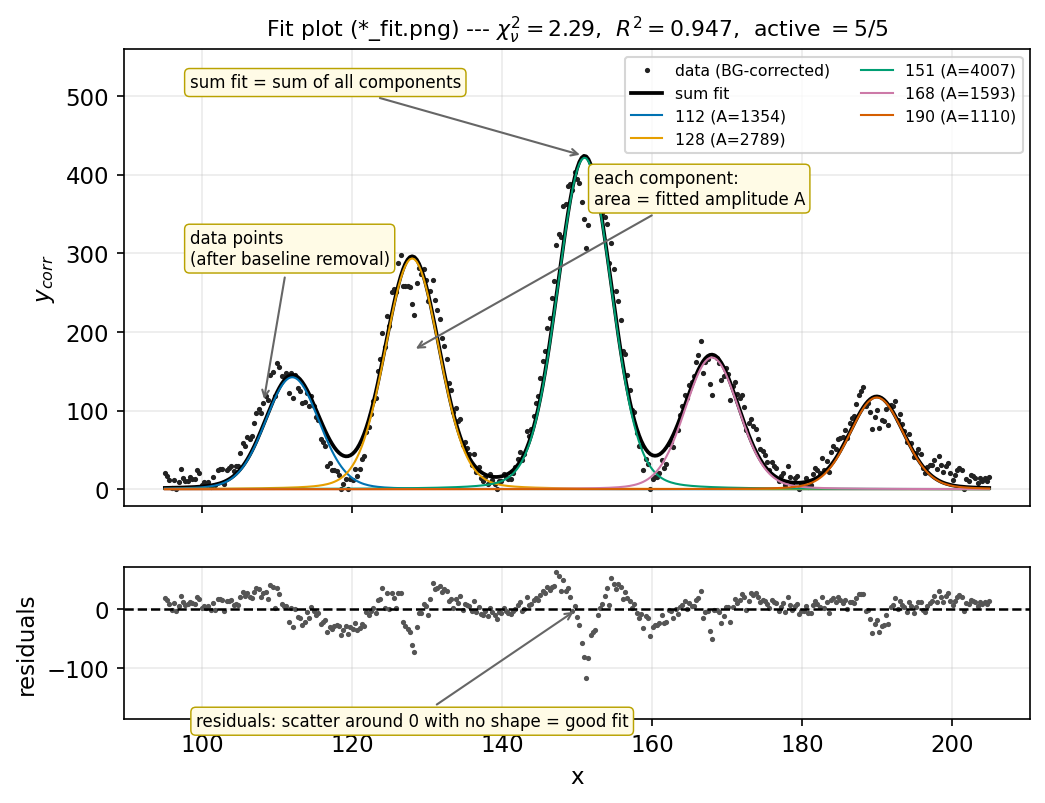
\includegraphics[width=0.92\linewidth]{figures/fig_fit_annotated.png}
\caption{How to read \code{*_fit.png}: the data after baseline removal, the summed
fit, the individual components (area $=$ amplitude), the goodness-of-fit summary in
the title, and the residual panel below.}
\label{fig:fit_annot}
\end{figure}

\begin{figure}[h]\centering
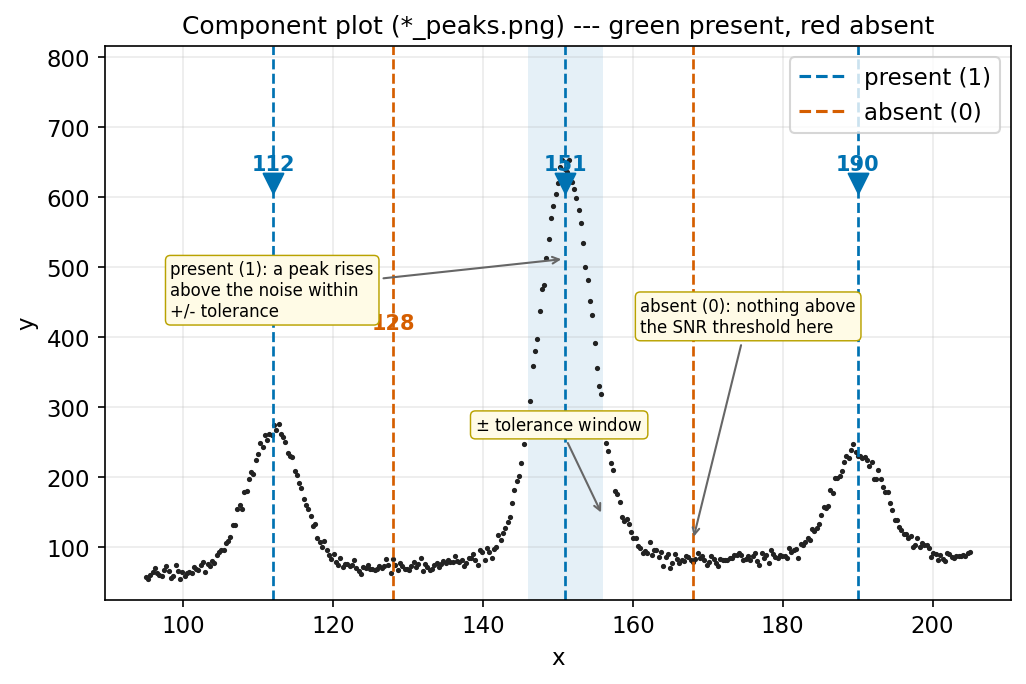
\includegraphics[width=0.92\linewidth]{figures/fig_presence_annotated.png}
\caption{How to read \code{*_peaks.png}: a green marker/line flags a peak that is
present ($1$), a red line one that is absent ($0$); the call is made within the
$\pm$\code{tolerance} window (shaded).}
\label{fig:presence_annot}
\end{figure}

\bigskip
% =====================================================================
\section{Troubleshooting \& FAQ}
\begin{description}
\item[The GUI does not start.] On a headless machine (no display) or without Tk,
use the command line: \code{peakcheck --config job.toml --no-gui}. On Debian/Ubuntu
install Tk with \code{sudo apt install python3-tk}.
\item[\textnormal{``\code{--no-gui needs a config file}''.}] Headless mode needs a
TOML (or at least \code{--reference}). Write one with
\code{peakcheck --write-template job.toml}.
\item[No peaks are found.] Lower \code{prominence_init} and/or \code{min_snr_init},
check the search window \code{x_min}/\code{x_max}, or simply click the peaks in the
GUI. Confirm the \emph{x conversion} so positions are in the units you expect.
\item[Reduced $\chi^2_\nu$ is far above 1.] The fixed-shape model is being
strained: the widths \code{wg}/\code{wl} probably do not match the data, or a peak
is missing. Add the missing peak or correct the widths; the amplitudes remain the
best non-negative fit.
\item[Peaks I placed disappear after the fit (active count drops), or the fit is
one broad hump.] The profile is far wider than the data's peaks, so the
overlapping profiles become redundant and the non-negative fit sets some
amplitudes to zero. Almost always the widths \code{wg}/\code{wl} are on the wrong
scale: e.g.\ they are instrumental values in cm\textsuperscript{-1} but the data
are still in meV because the \emph{x conversion} is off. Set the conversion (or
load the matching config), or set \code{wg}/\code{wl} to roughly your peaks'
half-width. PeakCheck prints a hint in this case. The marker labels and the fit
labels always show the same positions; only their displayed precision matches now
(one decimal), so a peak does not ``move'' between picking and fitting.
\item[A peak I expect is reported ``absent''.] Raise \code{tolerance} if the
component peak is shifted, or lower \code{snr_thresh} for a noisy component. Check
that \code{presence_baseline_corrected} matches your intent (height above baseline
vs.\ raw signal).
\item[The reported errors look wrong.] With a real error column the
\code{statistical} mode gives true $1\sigma$; without one, errors are scaled by
$\sqrt{\chi^2_\nu}$. Supply an error column for count data spanning orders of
magnitude. The supplement shows a Monte-Carlo check of the error budget.
\item[The file will not load.] PeakCheck reads two- or three-column whitespace or
CSV text and ignores comment lines beginning with \texttt{\#}, \texttt{!} or
\texttt{\%}; non-finite rows are dropped. Check the delimiter and the error-column
setting.
\item[Can I reproduce a run exactly?] Yes --- save the config (\emph{Save config},
Ctrl+S) or reuse the parameter block from the CSV header / Excel \code{Parameters}
sheet, and rerun with \code{--config}.
\end{description}

\noindent\rule{\linewidth}{0.4pt}\\[2pt]
{\footnotesize PeakCheck \textperiodcentered\ User Manual \textperiodcentered\
\textcopyright\ 2026 Lukas Knauer, RPTU Kaiserslautern-Landau, AG Sch\"unemann
\textperiodcentered\ The technical details of every computation step are in the
accompanying supplement.}

\end{document}
